\documentclass[../bryant_comp_sys.tex]{subfiles}

\begin{document}
\section{A Tour of Computer Systems}

    \begin{outline}
        \1 Traces the lifetime of a \texttt{hello.cpp} program from creation, runtime, output, through to termination.
    \end{outline}

    \lstset{language=C++}
    \begin{lstlisting}
        #include <stdio.h>

        int main()
        {
            printf(``hello, world\n'');
        }
    \end{lstlisting}

    \subsection{Information is Bits + Context}
        \begin{outline}
            \1 ASCII -- most common representation for text characters. Each character is represented by a byte-sized integer
            \1 ``All information in a system --- including disk files, programs stored in memory, user data stored in memory, and data transferred across a network --- is represented as a bunch of bits.'' (pg. 3)
        \end{outline}

    \subsection{Programs are Translated by Other Programs into Different Forms}
        \begin{outline}
            \1 Individual programs (such as in C) are translated by \textit{\glspl{compiler}} into machine--language instructions, stored as binary files (also called an \textit{executable}).
            \1 Four different phases of this process (using a C program as an example):
                \2 \textit{Preprocessing}: Modifies the original code according to directives begining with the \# character (such as \#include statements) and outputs a \texttt{.i} file.
                \2 \textit{Compilation phase}: Translates the preprocessed code into an \textit{\gls{assemblyLanguage}} program (a \texttt{.s} file). Important since this is a common output language for all compilers for all high--level languages (e.g. C and Fortran compilers output programs in the same assembly--language)
                \2 \textit{Assembly}: The assembly--language program is translated into \textit{\gls{machineLanguage}} instructions, called a \textit{relocatable program} (\texttt{.o} file)
                \2 \textit{Linking}: Links the program to external libraries (such as the C standard library) to output an \textit{executable object file}.
        \end{outline}

    \subsection{It Pays to Understand How Compilation Systems Work}
        \begin{outline}
            \1 Gives several reasons why it's important to understand how compilers work:
                \2 \textbf{Optimizing program performance}. Optimization of code relies on understanding how a compiler turns certain statements into machine--language (i.e. \texttt{switch} statements vs \texttt{if--else} statements)
                \2 \textbf{Understanding link--time errors}. What to certain link errors mean, how can we resolve them?
                \2 \textbf{Avoiding security holes}. Buffer overflow is one of the main source of vulnerabilities, so understanding data types and structures is important
        \end{outline}

    \subsection{Processors Read and Interpret Instructions Stored in Memory}
        \begin{outline}
            \1 At this point in our example, our program is compiled into an executable.
            \1 How do we run it? What happens to it when we do?
            \1 The shell is a base way humans interact with a computer. Run programs by typing \texttt{./\$PROGRAM}, where \texttt{\$PROGRAM} is the name of the executable.
        \end{outline}

        \subsubsection{Hardware Organization of a System}
            \begin{outline}
                \1 Many different, interacting parts go into a modern computer system (\Fref{fig:hardware_organization_1}).
                \begin{figure}
                    \centering
                    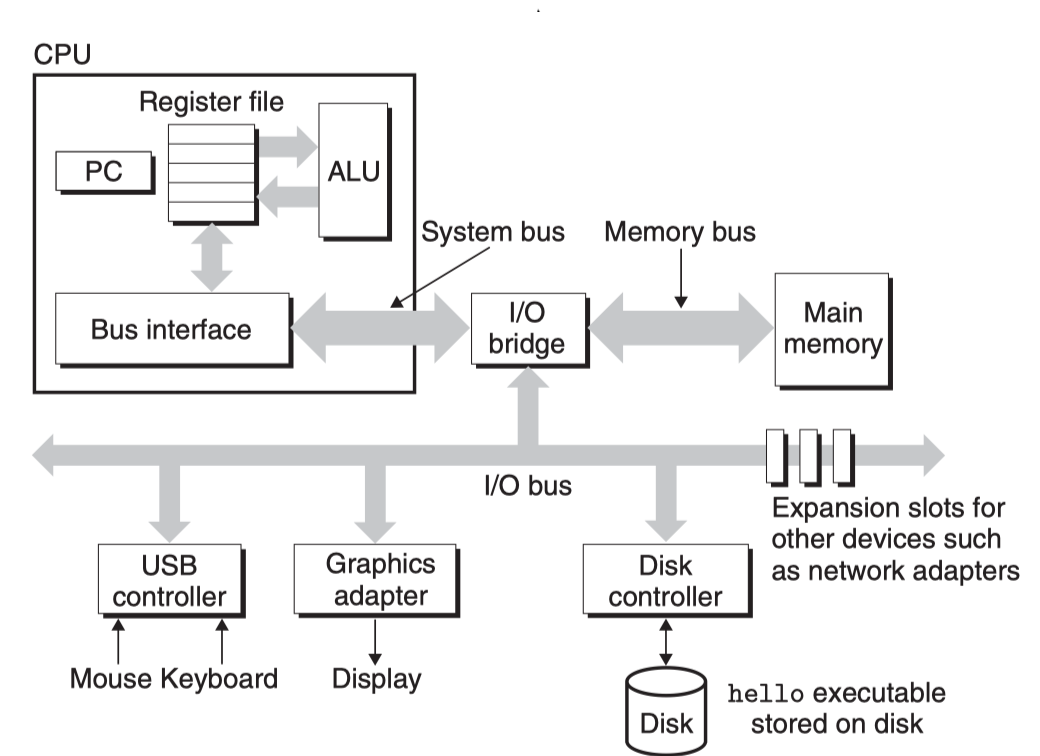
\includegraphics[width=0.5\linewidth]{ch1/figs/hardware_organization_1.png}
                    \label{fig:hardware_organization_1}
                    \caption{Organization of a modern computer system (pg. 8).}
                \end{figure}
                \1 This subsection goes through each of the subsystems in turn.
            \end{outline}

            \paragraph{Buses}
                \begin{outline}
                    \1 Each fixed--size chunk of bytes carried by a \gls{bus} is called a \textit{\gls{word}}, with a size of 4 bytes in 32 bit machines and 8 bytes in 64 bit machines (most modern machines are 64 bit)
                \end{outline}

            \paragraph{I/O Devices}
                \begin{outline}
                    \1 Connect the system to the external world (e.g. keyboard, mouse, etc.)
                    \1 Each I/O device is connected to the I/O bus using some type of controller, which are chips on the device or motherboard.
                \end{outline}

            \paragraph{Main Memory}
                \begin{outline}
                    \1 Volatile (i.e. temporary) memory (\gls{ram}) which holds programs and the data they manipulate. 
                    \1 Linear arrays of bytes, each with their own index (address), starting at index 0.
                    \1 The size of the data items stored in memory depend on their declared type (int, float, etc.) in whatever program it is that the memory belongs to.
                \end{outline}

            \paragraph{Processor}
                \begin{outline}
                    \1 The \gls{cpu} executes instructions stored in main memory.
                    \1 Contains a \gls{word}--sized storage device (also called a register) called a \gls{pc}, which points at an address in main memory containing some machine--language instructions.
                    \1 Reads the instruction from memory, interprets the bits, executes the instruction, then updates the PC to point to the next instruction (which may or may not be contiguous in memory)
                    \1 Only performs a few types of operations, revolving around the main memory, the \gls{register}, and the \gls{alu}:
                        \2 Load: Copy a byte or word from main memory into a register.
                        \2 Store: Copy a byte or word from a register into main memory.
                        \2 Operate: Copy the contents of two registers to the ALU, perform an arithmetic operation on the two words, store the result in a register.
                        \2 Jump: Extract a word from the instruction itself and copy it to the PC
                \end{outline}
        
        \subsubsection{Running the \texttt{hello} Program} \label{sec:runProgram}
            \begin{outline}
                \1 While typing \texttt{./hello} in the shell, each character is read into the register and stored in memory.
                \1 The shell then loads the executable into memory from the disk, without passing through the processor by going through the memory bus.
                \1 Once loaded into memory, the processor begins executing the machine--language instructions within the compiled code (some good figures on pages 11 and 12 showing each step of this process mapped out on copies of \Fref{fig:hardware_organization_1}).
            \end{outline}

        \subsubsection{Caches Matter}
            \begin{outline}
                \1 IMPORTANT: ``[...] a system spends a lot of its time moving information from one place to another.'' (pg. 12)
                \1 This information movement overhead slows down parts of the program which depend on it.
                \1 Larger storage devices are slower than smaller storage devices.
                \1 Register files store only a few hundred bytes of data while main memory holds billions, but a processor can read data from a register file almost 100 times faster than from main memory (called the \textit{processor--memory gap}).
                \1 To deal with this, there is a hierarchy of \glspl{cache} (see \Fref{fig:mem_hierarchy} for more) which serve as temporary staging areas for information.
                \1 Information can be staged in this cache hierarchy so the processor can more quickly access data.
            \end{outline}

        \subsubsection{Storage Devices Form a Hierarchy}
            \begin{outline}
                \1 Storage devices of all type in a computer form a \textit{memory hierarchy} (\Fref{fig:mem_hierarchy}).
                \1 As you move up the hierarchy, memory becomes faster to access at a higher monetary cost.
                \1 The storage at one level acts as a cache for the storage one rung below it.
            \end{outline}

            \begin{figure}
                \centering
                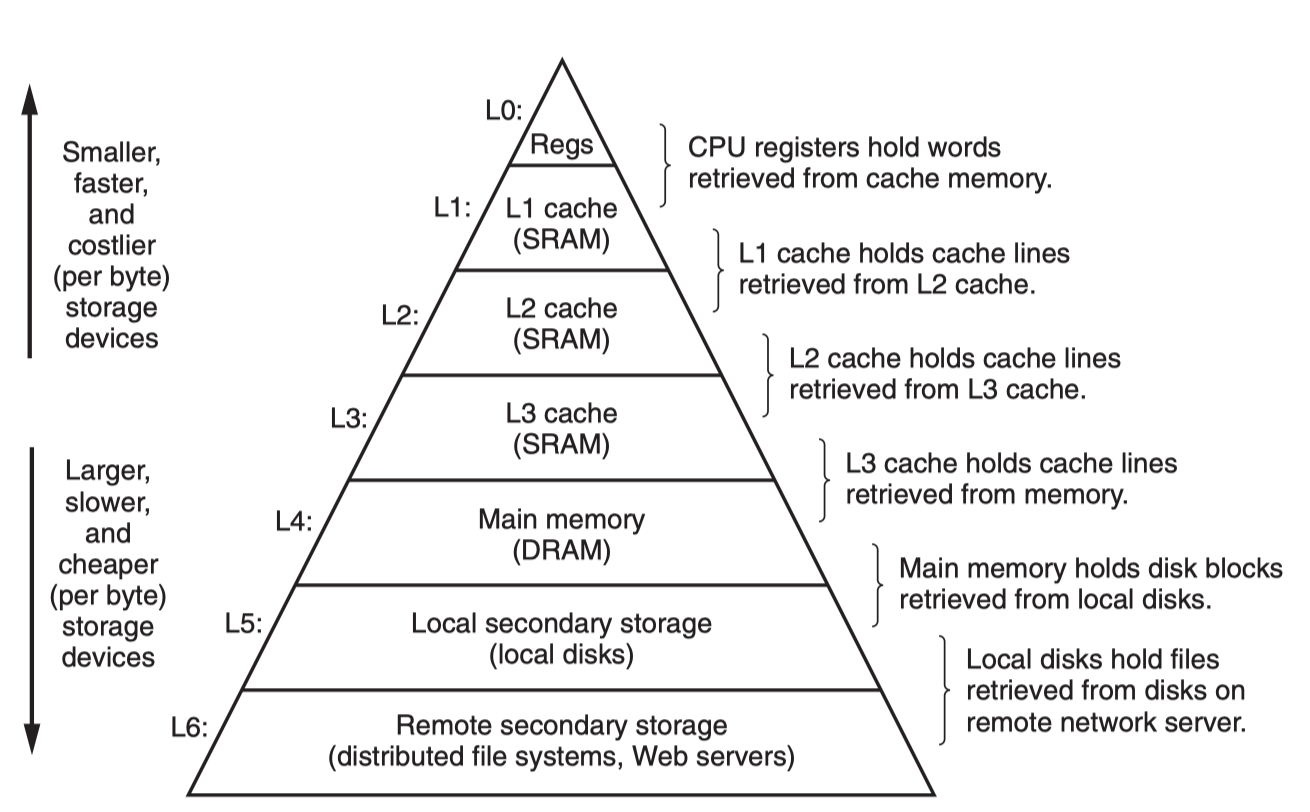
\includegraphics[width=0.5\linewidth]{ch1/figs/mem_hierarchy.png}
                \label{fig:mem_hierarchy}
                \caption{Example of a memory hierarchy.}
            \end{figure}

    \subsection{The Operating System Manages the Hardware}
        \begin{outline}
            \1 Note that when outlining running the program (\Fref{sec:runProgram}) the program itself never accessed the keyboard, display, disk, or main memory.
            \1 This is instead done by the computer's \gls{os}.
            \1 Operating systems have two main purposes:
                \2 Protect the hardware from runaway programs.
                \2 Provide higher--level, simple, and uniform mechanisms for interacting with low--level hardware.
            \1 An operating system has three fundamental abstractions: processes, virtual memory, and files.
        \end{outline}

        \subsubsection{Processes}
            \begin{outline}
                \1 A \gls{process} is the operating system's abstraction for a running program.
                \1 A single CPU can run multiple processes concurrently by switching between them (called \gls{context}). The CPU keeps track of all the information about a running processes, such as the register file, its data in main memory, etc., which is called a \textit{context}. The CPU can then switch between processes by storing one context, switching, and restoring the context (\Fref{fig:context_switching}).
                \1 A processes can contain multiple execution units called \textit{threads}, each running in the context of its umbrella processes and sharing the same code and data.
                \1 IMPORTANT: It is much easier to share data between multiple threads than it is between multiple processes (i.e. it is much easier to parallelize code in a multithreaded manner than in a multiprocessor manner).
            \end{outline}

            \begin{figure}
                \centering
                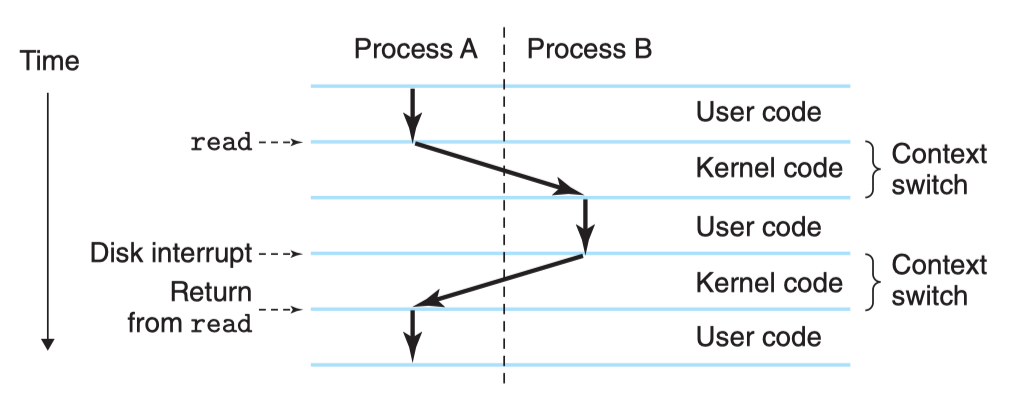
\includegraphics[width=0.5\linewidth]{ch1/figs/context_switching.png}
                \label{fig:context_switching}
                \caption{Minimal example of context switching between two concurrent processes.}
            \end{figure}

        \subsubsection{Virtual Memory}
            \begin{outline}
                \1 Abstraction that gives the illusion that each process has exclusive access to memory (see \gls{vmem})
                \1 Each process has the same view of memory, called the \textit{virtual address space}
                \1 Hierarchical: topmost for code and data common to all processes, lower region for code and data specific to user created processes (\Fref{fig:virtual_address_hierarchy})

                \begin{figure}
                    \centering
                    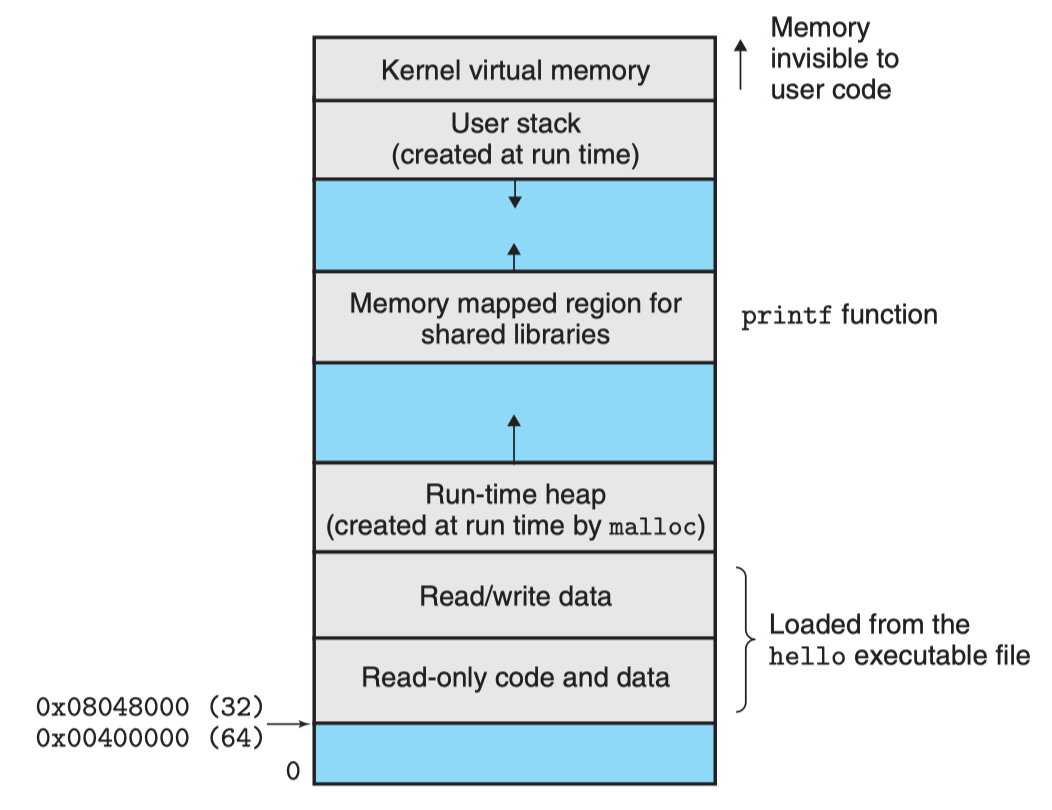
\includegraphics[width=0.5\linewidth]{ch1/figs/virtual_memory_hierarchy.png}
                    \label{fig:virtual_address_hierarchy}
                    \caption{Virtual address space hierarchy.}
                \end{figure}

                \1 Well--defined spaces of memory space (* denotes important concepts, which I've heard of before):
                    \2 \textbf{Program code and data}: Code begins at same address for all processes, followed by data that correspond to global C variables, initialized directly from the executable.
                    \2 \textbf{\Gls{heap}*}: Initialized at run--time. Expands and contracts as a result of memory allocation calls in whatever program it is that's running (e.g. C/Cpp's \texttt{malloc}).
                    \2 \textbf{Shared libraries}: Holds the code and data for shared libraries (e.g. C/Cpp's STL)
                    \2 \textbf{\Gls{stack}*}: Area where compiler implements function calls of a program. Expands with each function call and contracts when returned from the function.
                    \2 \textbf{Kernel virtual memory}: The part of the operating system which permanently resides in memory.
            \end{outline}

        \subsubsection{Files}
            \begin{outline}
                \1 ``A \textit{file} is a sequence of bytes, nothing more and nothing less.'' (pg. 19)
            \end{outline}

    \subsection{Concurrency and Parallelism}
        \begin{outline}
            \1 \Gls{parallelism} refers to using \gls{concurrency} to make code faster (i.e. running multiple, simultaneous activities/processes)
            \1 Three levels of abstraction:
        \end{outline}

        \subsubsection{Thread--Level Concurrency}
            \begin{outline}
                \1 The concept of using threads to run multiple control flows executing within a single processes.
                \1 \Gls{multcore}: Processors with multiple cores per chip.
                    \2 These cores have their own L1 and L2 cache, but share higher level caches and interfaces to main memory. 
                \1 \Gls{multthread}: Processors which allow multiple flows of control per core.
                    \2 Each core has multiple copies of some CPU hardware, such as registers and PCs, while sharing interfaces with other parts like ALUs.
                    \2 Multithreaded processors decide which thread to execute on a cycle--per--cycle basis.
                \1 Improves system performance in two ways:
                    \2 Reduces the need for single cores to simulate concurrency by context switching.
                    \2 Can run single applications faster, iff \textbf{the program is written such that it can utilize multiple threads effectively.}
            \end{outline}
        
        \subsubsection{Instruction--Level Parallelism}
            \begin{outline}
                \1 Refers to the ability of a processor to execute multiple instructions at once.
                \1 Each individual instruction can take longer, but a processor can execute 100s of instructions simultaneously
                \1 \Gls{pipelining}: when actions required to execute instructions are partitioned into discrete steps
                \1 Most modern processors are \textit{superscalar}, meaning they have execution rates faster than one instruction per cycle
            \end{outline}

        \subsubsection{\Gls{smid} Parallelism}
            \begin{outline}
                \1 Allows single instructions to trigger multiple operations run in parallel.
                \1 An example of this is the ability of modern processors to add four pairs of single--precision floating--point numbers at once
            \end{outline}
\end{document}